% Final defense deck (2026-12-13): 20 minutes + 5 minutes of questions, 15 slides,
% every slide assigned to one member in \note{} so that all four speak.
% Compile from this directory: pdflatex main.tex (twice). See ../README.md.
% Every number comes from data/raw/manifest.json, data/eval/questions.json,
% results/retrieval.csv, results/retrieval_questions.csv, README.md,
% docs/build-your-own-rag.md or a commit message. Missing numbers are \TODO{}.
% The two results tables are written by another script into docs/report/generated/
% and are read with \input when they exist.
\documentclass[12pt,aspectratio=169]{beamer}
\usetheme[progressbar=frametitle,numbering=fraction]{metropolis}
\usepackage[T1]{fontenc}
\usepackage[sfdefault]{FiraSans}
\usepackage[scale=0.85]{FiraMono}
\usepackage{booktabs}
\usepackage{adjustbox}
\usepackage{tikz}
\usetikzlibrary{arrows.meta,positioning,fit,backgrounds}

\newcommand{\TODO}[1]{\textcolor{red}{\textbf{TODO:} #1}}
\newcommand{\gendir}{../../report/generated}
% \slidetable{file}{todo}: input a generated results table, scaled to the slide width.
% The generated files are table floats with a long caption (for the report): on a
% slide the float wrapper and the caption are dropped, and the tabular is resized.
\newcommand{\slidetable}[2]{%
  \IfFileExists{#1}{%
    \begingroup
      \renewenvironment{table}[1][]{\ignorespaces}{\unskip}%
      \renewcommand{\caption}[2][]{\ignorespaces}%
      \renewcommand{\label}[1]{\ignorespaces}%
      \resizebox{\linewidth}{!}{\input{#1}\unskip}%
    \endgroup
  }{\TODO{#2}}}
\setbeamertemplate{note page}[plain]
% Metropolis draws the title page in a box of \paperheight, which is reported as an
% overfull \vbox on every deck; the same layout in a shorter box fits.
\makeatletter
\setbeamertemplate{title page}{%
  \begin{minipage}[c][0.85\textheight]{\textwidth}
    \vfill
    \usebeamertemplate*{title}
    \usebeamertemplate*{subtitle}
    \usebeamertemplate*{title separator}
    \usebeamertemplate*{author}
    \usebeamertemplate*{date}
    \usebeamertemplate*{institute}
    \vfill
  \end{minipage}}
\makeatother

\title{Trustworthy RAG on Medical Documents}
\subtitle{Cited answers from WHO guidelines and PubMed OA articles, with a refusal gate}
\author{Boussoualim Yassine \and Benahcene Mohamed Wassim \and Aissaoui Anes Safouane \and Djerdali Mohamed Achraf}
\setbeamerfont{author}{size=\small}
\setbeamerfont{date}{size=\small}
\institute{LLM Final Projects 2026--2027, Prof.\ A.\ Moussaoui, Project 2\\
  Group \TODO{group number} \quad \TODO{school}}
\date{Oral defense, 13 December 2026}

% Architecture as built (src/ingest.py, index.py, bm25.py, rag.py, rerank.py, app.py).
\newcommand{\archfigure}{%
\begin{tikzpicture}[
    box/.style={draw=black!60, rounded corners=3pt, fill=##1, align=center,
                text width=2.1cm, minimum height=1.5cm, font=\footnotesize,
                execute at begin node={\hyphenpenalty=10000\relax}},
    box/.default=black!5,
    arr/.style={-{Stealth[length=2.2mm]}, thick, black!70},
    lab/.style={font=\footnotesize\bfseries, black!70, anchor=south west, inner sep=1pt}]
  % offline row
  \node[box] (docs)  at (0,0)   {50 docs\\20 WHO PDF\\30 PMC text};
  \node[box] (chunk) at (2.5,0) {Chunks\\512 tokens\\102 overlap};
  \node[box] (emb)   at (5,0)   {Embed\\BGE-M3};
  \node[box] (store) at (7.5,0) {Chroma\\(cosine)\\+ BM25};
  \draw[arr] (docs) -- (chunk);
  \draw[arr] (chunk) -- (emb);
  \draw[arr] (emb) -- (store);
  \node[lab] at (docs.north west) [yshift=2pt] {Offline: build the index once};
  % online row
  \node[box=blue!8]    (q)     at (0,-2.65)    {Question};
  \node[box=blue!8]    (ret)   at (2.5,-2.65)  {Dense 20\\BM25 20\\RRF: top 5};
  \node[box=orange!15] (gate)  at (5,-2.65)    {Gate\\MiniLM\\score $\geq 0.5$?};
  \node[box=blue!8]    (llm)   at (7.5,-2.65)  {Free LLM\\passages\\{[}1{]}--{[}5{]}};
  \node[box=orange!15] (check) at (10,-2.65)   {Citation\\check};
  \node[box=green!12]  (ans)   at (12.5,-2.65) {Answer\\{[}source, p.\,N{]}};
  \draw[arr] (q) -- (ret);
  \draw[arr] (ret) -- (gate);
  \draw[arr] (gate) -- (llm);
  \draw[arr] (llm) -- (check);
  \draw[arr] (check) -- (ans);
  \draw[arr] (store.south) .. controls +(0,-0.8) and +(0.6,0.8) .. (ret.north east);
  \node[box=red!10, text width=6.6cm, minimum height=0.9cm] (ref) at (7.5,-4.7)
     {Refusal: \emph{``I cannot answer this question from the provided documents.''}};
  \draw[arr] (gate.south) -- node[left, font=\footnotesize] {no} (gate.south |- ref.north);
  \draw[arr] (check.south) -- node[right, font=\footnotesize] {fail} (check.south |- ref.north);
  \begin{scope}[on background layer]
    \node[draw=blue!40, dashed, rounded corners, inner sep=5pt,
          fit=(q) (ans) (ref)] (app) {};
  \end{scope}
  \node[lab] at (app.north west) [yshift=1pt] {Online, in the Gradio app};
\end{tikzpicture}}

% Score lines of the two refusal gates, original 30 questions (results/retrieval_questions.csv).
\newcommand{\gatefigure}{%
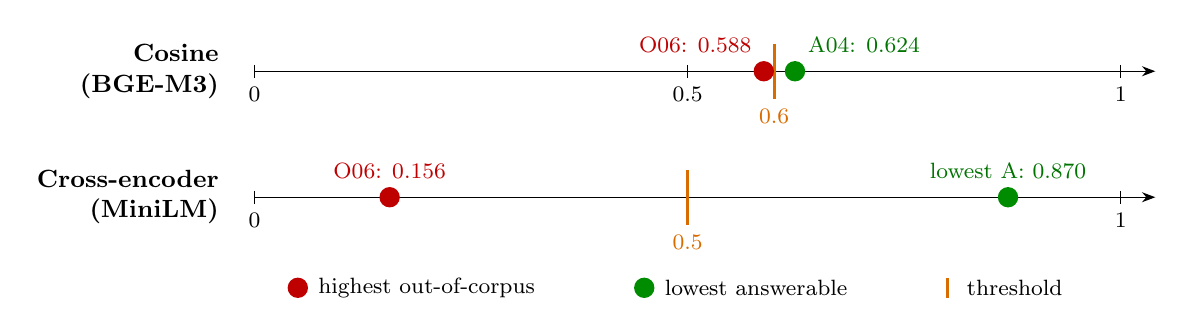
\begin{tikzpicture}[x=11cm, font=\small,
    dotA/.style={circle, fill=green!55!black, inner sep=2.6pt},
    dotO/.style={circle, fill=red!75!black, inner sep=2.6pt},
    thr/.style={very thick, orange!85!black}]
  % cosine similarity, BGE-M3
  \node[anchor=east, align=right, font=\small\bfseries] at (-0.03,0) {Cosine\\(BGE-M3)};
  \draw[-{Stealth}] (0,0) -- (1.04,0);
  \foreach \x in {0,0.5,1} \draw (\x,0.08) -- (\x,-0.08) node[below, font=\footnotesize] {\x};
  \draw[thr] (0.6,0.35) -- (0.6,-0.35) node[below, font=\footnotesize] {0.6};
  \node[dotO] at (0.588,0) {};
  \node[dotA] at (0.624,0) {};
  \node[red!75!black, anchor=south east, font=\footnotesize] at (0.585,0.12) {O06: 0.588};
  \node[green!45!black, anchor=south west, font=\footnotesize] at (0.628,0.12) {A04: 0.624};
  % cross-encoder, MiniLM, sigmoid
  \begin{scope}[yshift=-1.6cm]
  \node[anchor=east, align=right, font=\small\bfseries] at (-0.03,0) {Cross-encoder\\(MiniLM)};
  \draw[-{Stealth}] (0,0) -- (1.04,0);
  \foreach \x in {0,1} \draw (\x,0.08) -- (\x,-0.08) node[below, font=\footnotesize] {\x};
  \draw[thr] (0.5,0.35) -- (0.5,-0.35) node[below, font=\footnotesize] {0.5};
  \node[dotO] at (0.156,0) {};
  \node[dotA] at (0.870,0) {};
  \node[red!75!black, anchor=south, font=\footnotesize] at (0.156,0.12) {O06: 0.156};
  \node[green!45!black, anchor=south, font=\footnotesize] at (0.870,0.12) {lowest A: 0.870};
  \end{scope}
  % legend
  \node[dotO, label={[font=\footnotesize]right:highest out-of-corpus}] at (0.05,-2.75) {};
  \node[dotA, label={[font=\footnotesize]right:lowest answerable}] at (0.45,-2.75) {};
  \draw[thr] (0.8,-2.62) -- (0.8,-2.88) node[right, font=\footnotesize, black] at (0.81,-2.75) {threshold};
\end{tikzpicture}}

\begin{document}

\begin{frame}
  \titlepage
  \note{Speaker: Boussoualim Yassine. Opens: names the four members and who presents which part, then hands over to Achraf.}
\end{frame}

\begin{frame}{The problem}
  \begin{itemize}
    \item An LLM alone answers from memory
    \item A wrong dose sounds as sure as a right one
    \item We want: answers \alert{only} from trusted documents
    \item Every claim shows its source
    \item No evidence $\Rightarrow$ refuse:\\
      \emph{``I cannot answer this question from the provided documents.''}
  \end{itemize}
  \note{Speaker: Djerdali Mohamed Achraf. Retrieval always returns five passages, even for ``Who painted the Mona Lisa?'' (O09), so refusing has to be designed, not hoped for.}
\end{frame}

\begin{frame}{State of the art}
  \small
  \begin{tabular}{@{}ll@{}}
    \toprule
    Idea & Reference \\
    \midrule
    Retrieve, then generate (RAG) & Lewis et al., 2020 \\
    Keyword ranking: BM25 & Robertson \& Zaragoza, 2009 \\
    Dense embeddings: BGE-M3 & Chen et al., 2024 \\
    Rank fusion: RRF & Cormack et al., 2009 \\
    Cross-encoder rerankers & Nogueira \& Cho, 2019; MedCPT 2023 \\
    RAG metrics & RAGAS, Es et al., 2023 \\
    \bottomrule
  \end{tabular}
  \bigskip

  \normalsize Our angle: \alert{checked citations} + \alert{refusal gate} + held-out refusal test
  \note{Speaker: Aissaoui Anes Safouane. We reuse known pieces; what we add is the checking around them. Full references are in the report.}
\end{frame}

\begin{frame}{Data: 50 documents}
  \begin{tabular}{@{}lll@{}}
    \toprule
    Source & Count & Size \\
    \midrule
    WHO guidelines (PDF, WHO IRIS) & 20 & 25.9\,MB \\
    PubMed Central OA (full text) & 30 & 1.3\,MB \\
    \bottomrule
  \end{tabular}
  \bigskip
  \begin{itemize}
    \item Hypertension, diabetes, TB, malaria, HIV, antenatal care, paracetamol
    \item 1530 records (1500 WHO pages) $\to$ 3410 chunks
    \item Chunks: 512 tokens, 102 overlap
  \end{itemize}
  \note{Speaker: Boussoualim Yassine. Sizes are the byte totals of data/raw/manifest.json, which records the URL of every file; fetch\_corpus.py --from-manifest downloads the same corpus. PubMed articles come as text because Europe PMC refuses PDFs to scripts. A WHO chunk keeps its page number for the citation.}
\end{frame}

\begin{frame}{Pipeline}
  \centering
  \adjustbox{max width=\linewidth, max height=0.74\textheight}{\archfigure}
  \note{Speaker: Boussoualim Yassine. Offline: BGE-M3 embeddings in Chroma, resumable build (about 3 hours on a laptop CPU). BM25 is built in memory from the same chunks. Online: 20 dense + 20 BM25 candidates fused by RRF, top 5 passages, then the gate, the free LLM and the citation check. Two places can refuse.}
\end{frame}

\begin{frame}{BM25 from scratch}
  \small
  \[
    \mathrm{score}(q,d)=\sum_{t\in q}\mathrm{idf}(t)\,
      \frac{tf\,(k_1+1)}{tf+k_1\,(1-b+b\,\frac{dl}{avgdl})}
    \qquad k_1=1.5,\; b=0.75
  \]
  \[
    \mathrm{idf}(t)=\ln\Big(1+\frac{N-df+0.5}{df+0.5}\Big)
  \]
  \normalsize
  \begin{itemize}
    \item Standard library only: inverted index, no search package
    \item Evidence page found: dense 0.80, \alert{BM25 0.95}, hybrid 0.90
    \item BM25 score has no fixed scale $\Rightarrow$ it does not gate
  \end{itemize}
  \note{Speaker: Boussoualim Yassine. Page hit rates from results/retrieval.csv (20 answerable questions). The +1 inside the log keeps idf positive (Lucene's variant of Robertson and Zaragoza). Built following two build-your-own-x tutorials, cited in the code and the report. BM25 helps with exact names such as zilebesiran (A16).}
\end{frame}

\begin{frame}{Refusal gate}
  \centering
  \adjustbox{max width=0.9\linewidth}{\gatefigure}
  \medskip
  \begin{itemize}\small
    \item Cosine measures topic: near-topic questions come close
    \item Cross-encoder reads question + passage together
    \item 0.5 is the model's own boundary: \alert{not tuned} on our questions
  \end{itemize}
  \note{Speaker: Aissaoui Anes Safouane. O06 is isotretinoin for acne: cosine refuses it by only 0.012, and 0.6 was checked on the same 30 questions. The cross-encoder gives it 0.156. Both scores rank every answerable question above every out-of-corpus one (auroc 1.0), so the difference is the untuned threshold and the margin. Measured on the original 30 questions. The gate stops at the first passage that reaches 0.5: about 0.3 s for an answered question, 0.5 s for a refused one.}
\end{frame}

\begin{frame}{Citation check}
  \begin{itemize}
    \item Passages numbered [1]--[5] in the prompt
    \item Keep the reply only if it cites $\geq 1$ passage, all within [1]--[5]
    \item {[}2{]} $\to$ \texttt{[WHO\_09\ldots, p.\,14]} or \texttt{[article title]}
    \item Otherwise: refusal
  \end{itemize}
  \medskip
  \small
  \begin{tabular}{@{}ll@{}}
    \toprule
    Reply & Verdict \\
    \midrule
    ``\ldots at least 24 hours [1].'' & \texttt{answered} \\
    ``\ldots at least 24 hours.'' & \texttt{uncited} \\
    ``\ldots [3]'' with 2 passages & \texttt{uncited} \\
    the refusal sentence & \texttt{model\_refused} \\
    \bottomrule
  \end{tabular}
  \note{Speaker: Aissaoui Anes Safouane. Reference markers inside articles, like [12], are rewritten to (12) in the prompt so they cannot pass as citations. Limit: the check proves the numbers exist, not that the passage supports the claim; faithfulness (LLM judge) measures that.}
\end{frame}

\begin{frame}{Evaluation setup}
  \begin{columns}[T]
    \begin{column}{0.44\linewidth}
      \textbf{40 questions}
      \begin{itemize}\small
        \item 20 answerable (A)
        \item 10 out-of-corpus (O)
        \item 10 held-out, near-domain (N)
      \end{itemize}
    \end{column}
    \begin{column}{0.54\linewidth}
      \textbf{5 systems}
      \begin{itemize}\small
        \item \texttt{rag\_dense}, \texttt{rag\_hybrid}, \texttt{rag\_rerank}
        \item baselines: \texttt{bm25\_rag}, \texttt{no\_rag}
      \end{itemize}
    \end{column}
  \end{columns}
  \bigskip
  \small
  \textbf{Metrics:} answer rate, refusal rate (O, N), hit rate, context precision,
  faithfulness (LLM judge), human \texttt{correct\_0\_1}\\[0.5em]
  \textbf{Models:} \texttt{nemotron-3-ultra} (all systems), \texttt{gemma-4-31b} (\texttt{rag\_rerank})
  \note{Speaker: Benahcene Mohamed Wassim. A questions have a ground truth, page and verbatim quote; 20/20 quotes are found in the corpus. O: 7 medical, 3 general knowledge. N questions are on corpus topics but ask facts the corpus lacks; they were committed before any result and no threshold was chosen with them. Free models only: 50 requests a day, so the run is resumable and caches every reply.}
\end{frame}

\begin{frame}{Results: retrieval (no LLM call)}
  \centering
  \slidetable{\gendir/retrieval_table.tex}{docs/report/generated/retrieval\_table.tex (written by the report script)}
  \medskip

  \small MiniLM gate: answers 20/20, refuses 10/10 at its own 0.5
  \note{Speaker: Benahcene Mohamed Wassim. Original 30 questions. Hybrid: page hit rate 0.90, hit rate 1.0, context precision 0.911, 0.16 s per question. Reordering with a cross-encoder did not pay: bge-reranker finds one more evidence page but takes about 50 s per question, so the cross-encoder only gates. MedCPT lets ``Who painted the Mona Lisa?'' through (0.78).}
\end{frame}

\begin{frame}{Results: five systems}
  \centering
  \slidetable{\gendir/summary_table.tex}{docs/report/generated/summary\_table.tex (after the evaluation run)}
  \medskip

  \small
  \TODO{two takeaways: \texttt{rag\_rerank} vs \texttt{no\_rag} and \texttt{bm25\_rag}
  (answer, refusal and held-out refusal rates); human \texttt{correct\_0\_1}}
  \note{Speaker: Benahcene Mohamed Wassim. Read the delta against the two baselines first, then the held-out refusal rate, which is the only refusal test the gates were not chosen on. Faithfulness is judged by the same model as the default generator.}
\end{frame}

\begin{frame}{Error analysis}
  \small
  \begin{tabular}{@{}lll@{}}
    \toprule
    Case & What went wrong & Response \\
    \midrule
    O06 isotretinoin & near miss: cosine 0.588 vs 0.6 & cross-encoder: 0.156 \\
    O09 Mona Lisa & MedCPT gate lets it through & MiniLM gate \\
    O04 multiple sclerosis & bge gate lets it through & MiniLM gate \\
    A19 & reasoning used all 600 tokens & resend once, 4000 \\
    citation check (toy) & cited passage lacks the claim & faithfulness judge \\
    \bottomrule
  \end{tabular}
  \bigskip

  \TODO{5--10 failures from the final run (records.jsonl, human rating sheet)}
  \note{Speaker: Benahcene Mohamed Wassim. MedCPT gives the Mona Lisa question 0.78, bge-reranker gives the multiple sclerosis question 0.85. A19: the default model is a reasoning model and returned no text within 600 tokens. The citation example is the toy reply in the tutorial that cites passage 1 for a fever claim it does not contain.}
\end{frame}

\begin{frame}{Ethics and limits}
  \begin{itemize}
    \item \alert{Not medical advice}: disclaimer on every answer
    \item No diagnosis; doses quoted, check with a clinician
    \item No patient data; questions go to OpenRouter
    \item Guidelines age: the corpus is a snapshot
    \item 50 documents, 40 questions: small
    \item Gate trained on web search; judge = generator model
  \end{itemize}
  \note{Speaker: Djerdali Mohamed Achraf. Never type anything that identifies a patient. Relevance is labelled per source document, so another document that also answers counts as a miss. Free models only, rate-limited.}
\end{frame}

\begin{frame}{Live demo}
  \small
  App: \texttt{http://127.0.0.1:7860}, mode \emph{Hybrid + cross-encoder gate}
  \medskip

  \textbf{1. Answerable (A06)}\\
  \texttt{How long should parenteral artesunate be given to a patient with severe malaria?}\\
  $\to$ at least 24\,h, until oral treatment is tolerated; WHO malaria guideline, p.\,79
  \medskip

  \textbf{2. Out of corpus (O06)}\\
  \texttt{How long is a typical course of isotretinoin for severe acne?}\\
  $\to$ refusal; cross-encoder 0.16, below 0.5
  \medskip

  Backup: \TODO{demo\_video.mp4}
  \note{Speaker: Djerdali Mohamed Achraf. Before the defense: index built, key in .env, free requests left today. Show the sources table and the Cited column for question 1, and the refusal reason for question 2 (the model is not called). If the network fails, play the video.}
\end{frame}

\begin{frame}{Conclusion}
  \begin{itemize}
    \item Built: hybrid retrieval, refusal gate, checked citations, BM25 from scratch, app
    \item Measured: \TODO{headline result against \texttt{no\_rag} and \texttt{bm25\_rag}}
    \item Next: check each claim against its passage; more held-out questions
  \end{itemize}
  \vfill
  \centering\Large Thank you. Questions?
  \note{Speaker: Djerdali Mohamed Achraf. Then the four members take questions on their own parts.}
\end{frame}

\end{document}
